% ID: SEL-D0009-BA-E01
% ESTADO: validada. S010; tres pasadas del mismo autor y comprobación matemática; sin segundo revisor.
\textbf{a) Formulación del modelo, sin resolverlo.}\par\nopagebreak[4]
Sean $x$ e $y$ los números de paquetes A y B. Expresamos las existencias en gramos: $3.75$ kg son $3750$ g y $4$ kg son $4000$ g. Cada restricción compara consumo y disponibilidad de un mismo recurso:
\[
\begin{cases}
75x+75y\leq3750 &\text{(arándanos)},\\
100x+50y\leq4000 &\text{(frambuesas)},\\
x\leq2y &\text{(límite de paquetes A)},\\
x\geq0,\quad y\geq0.
\end{cases}
\]
La función que se maximiza con los importes unitarios dados es
\[
\boxed{\max F(x,y)=2.40x+1.80y.}
\]
Las dos primeras restricciones se simplifican a $x+y\leq50$ y $2x+y\leq80$. Al contar paquetes completos se exige además $x,y\in\mathbb Z$; el modelo lineal continuo usa las mismas restricciones sin esta condición. No se inventan costes ausentes del enunciado. Este apartado pide formular \emph{sin resolver}: no calculamos aquí el óptimo.

\textbf{b) Región distinta y mínimo de la función indicada.}\par\nopagebreak[4]
Ahora se trabaja con las restricciones de este apartado, no con las anteriores:
\[
y\geq\frac{5-x}{4},\qquad y\geq\frac{4-x}{2},\qquad
y\leq\frac{35-7x}{5},\qquad x\geq0.
\]
La intersección de los semiplanos es un cuadrilátero cerrado y acotado. Sus vértices, en orden, son
\[
(0,2),\quad(3,1/2),\quad(5,0),\quad(0,7).
\]
Los dos vértices intermedios salen de igualar las fronteras primera/segunda y primera/tercera. En $x=0$ se obtiene $2\leq y\leq7$. La intersección de las fronteras segunda/tercera, $(50/9,-7/9)$, incumple la primera y se descarta. No se añade una restricción $y\geq0$ que el enunciado no da.
\begin{center}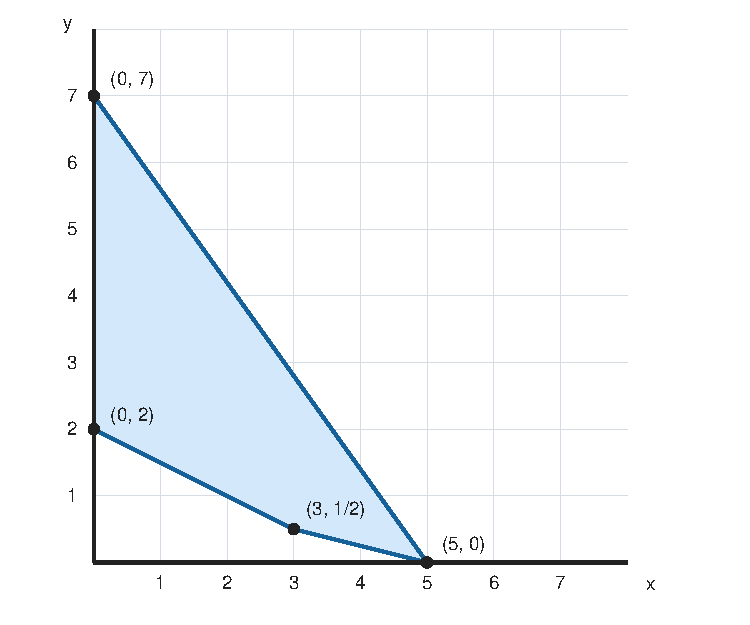
\includegraphics[width=0.58\linewidth]{recursos/figuras/s010-region.pdf}\end{center}
Una función lineal en un polígono alcanza sus extremos en algún vértice. Evaluamos:
\[
\begin{array}{c|rrrr}
(x,y)&(0,2)&(3,1/2)&(5,0)&(0,7)\\\hline
2x+y&2&13/2&10&7
\end{array}
\]
\boxed{F_{\min}=2\text{, únicamente en }(0,2).}
La unicidad se sigue también de que todo punto del polígono es combinación convexa de vértices y los otros tres valores son estrictamente mayores.
